\newpage
\chapter{TINJAUAN PUSTAKA} \label{Bab II}

\section{Tinjauan Pustaka} \label{II.Tinjauan}
Subbab ini menyajikan tinjauan pustaka yang bertujuan memberikan landasan teoretis bagi penelitian ini. Referensi yang digunakan diambil dari penelitian-penelitian serupa yang telah dilakukan sebelumnya sebagai dasar untuk penelitian ini. \par
\renewcommand{\arraystretch}{1.0} % Mengatur spasi antar baris menjadi 1

Pada penelitian yang dilakukan oleh O. Reyad, H.I. Shehata, dan M.E. Karar (2023), mengangkat permasalahan tentang jatuh sebagai salah satu peristiwa berbahaya yang sering dialami lansia, dengan data \textit{World Health Organization} (WHO) menunjukkan sekitar 30\% orang berusia di atas 65 tahun mengalami minimal satu kali jatuh per tahun, meningkat hingga 50\% untuk usia di atas 80 tahun. Peneliti mengembangkan arsitektur \textit{Internet of Health Things (IoHT)} dengan sistem deteksi jatuh berbasis \textit{ensemble machine learning}, khususnya model \textit{multi-stage random forest}. Metodologi penelitian menggunakan dataset \textit{SmartFall} yang mengumpulkan data dari \textit{accelerometer} tiga sumbu pada \textit{smartwatch}, kemudian membandingkan model yang diusulkan dengan tiga model \textit{machine learning} lainnya: \textit{K-nearest neighbors (KNN)}, \textit{decision tree (DT)}, dan \textit{standard random forest (SRF)}. Hasil penelitian menunjukkan bahwa model \textit{ensemble random forest} yang diusulkan mencapai akurasi tertinggi sebesar 98,4\%, mengungguli model \textit{machine learning} lainnya dalam deteksi jatuh pada lansia \cite{Reyad2023}. \par

Sementara itu, Penelitian yang berjudul \textit{Human Fall Detection from Sequences of Skeleton Features using Vision Transformer} oleh A Raza et al (2023), mengatasi tantangan ketergantungan metode deteksi jatuh konvensional pada sensor \textit{depth} (seperti \textit{Kinect}) dan model berbasis LSTM/CNN yang memerlukan komputasi intensif. Permasalahan utama termasuk keterbatasan akurasi dalam lingkungan dengan variasi pencahayaan, oklusi, serta kebutuhan akan sistem non-intrusif yang menjaga privasi pengguna dengan memanfaatkan data \textit{skeleton}. Metode yang diusulkan menggabungkan \textit{BlazePose} (untuk ekstraksi 33 titik \textit{skeleton} dari video RGB) dengan \textit{multi-headed transformer encoder} yang memproses urutan fitur \textit{skeleton}. Preprocessing menggunakan normalisasi posisi relatif (RP) dan interpolasi linear untuk mengatasi titik \textit{skeleton} yang hilang (reduksi dari 22,38\% menjadi 1,8\%). Hasil eksperimen pada dataset \textit{UR-FALL} dan \textit{UP-FALL} menunjukkan akurasi masing-masing 96,12\% dan 97,36\%, mengungguli metode berbasis CNN (95\%) dan LSTM (91,07\%) \cite{Raza2023}. \par

Kemudian penelitian berjudul "\textit{Pose-Based Fall Detection System: Efficient Monitoring on Standard CPUs}" oleh V. Mali dan S. Jaiswal (2024) mengatasi permasalahan ketergantungan sistem deteksi jatuh konvensional pada sensor \textit{wearable}, \textit{pressure mat}, atau model CNN berbasis GPU yang mahal dan tidak praktis untuk implementasi di panti jompo. Penelitian ini mengusulkan sistem non-intrusif berbasis \textit{pose estimation} menggunakan \textit{MediaPipe} untuk ekstraksi 33 \textit{landmark} tulang dari video \textit{RGB}. Metode utama meliputi analisis fitur berbasis \textit{threshold} (rasio tinggi badan, sudut torso-kaki, jarak kepala-lantai) dan mekanisme voting 20-frame buffer untuk meminimalkan \textit{false positive}. Hasil pengujian pada dataset GMDCSA24 (130 video aktivitas lansia) menunjukkan akurasi 91,54\%, presisi 88,24\%, dan recall 98,68\%, dengan spesifisitas 81,48\%. Sistem ini berjalan pada CPU standar tanpa memerlukan GPU atau sensor tambahan, menjadikannya solusi hemat biaya untuk fasilitas perawatan lansia \cite{Mali2025}. \par

Terdapat juga Penelitian yang berjudul "\textit{Vision-Based Fall Detection Using Dense Block With Multi-Channel Convolutional Fusion Strategy}" oleh X. Cai et al (2021) mengatasi masalah kehilangan informasi pada jaringan \textit{neural} dalam untuk deteksi jatuh berbasis visi. Permasalahan utama terletak pada degradasi informasi selama propagasi fitur di lapisan jaringan yang dalam, yang mengurangi kemampuan ekstraksi fitur dan menurunkan akurasi deteksi. Untuk mengatasi hal ini, penulis mengusulkan arsitektur MCCF-DenseBlock (Multi-Channel Convolutional Fusion Dense Block) yang menggabungkan koneksi padat (dense connections) dengan strategi fusi konvolusional multi-saluran. Arsitektur ini dilengkapi improved transition layer untuk mengurangi redundansi data melalui \textit{multi-level downsampling}. Hasil eksperimen menggunakan \textit{UR Fall Dataset} menunjukkan kinerja superior dengan F-score 0.973, mengungguli lima metode pembanding: dua berbasis fitur hand-crafted (GLR-FD dan MEWMA-FD) dan tiga berbasis deep learning (CNN-FD, Bi-LSTM-FD, CNN-LSTM-FD) \cite{Cai2021}. \par

Terakhir, Penelitian berjudul \textit{Fall Detection Method for Infrared Videos Based on Spatial-Temporal Graph Convolutional Network} oleh J. Yang et al (2024) mengatasi permasalahan keterbatasan kamera cahaya tampak (RGB) dalam deteksi jatuh, terutama terkait pelanggaran privasi, adaptasi lingkungan rendah cahaya, dan akurasi yang tidak optimal. Penulis mengusulkan metode berbasis video inframerah (\textit{near-infrared}/NIR dan \textit{thermal-infrared}/TIR) yang menggabungkan \textit{AlphaPose} untuk ekstraksi kerangka tubuh 2D dan jaringan \textit{Spatial-Temporal Graph Convolutional Network} (ST-GCN) yang dimodifikasi. Modifikasi ST-GCN meliputi strategi partisi spasial yang diperluas (\textit{expanded spatial partitioning}), unit konvolusi temporal multi-skala, serta representasi kerangka dalam sistem koordinat Kartesius dan polar. Hasil eksperimen pada dataset \textit{IR-Fall} (\textit{self-collected}) menunjukkan akurasi tertinggi 96.37\%, sedangkan pada dataset publik NTU-RGB+D-120 mencapai 94.64\%, mengungguli metode GCN lain seperti ST-GCN dasar (95.00\% pada \textit{IR-Fall}), CPS-GCN (95.35\%), dan AS-GCN (94.67\%). Metode ini juga dioptimalkan untuk \textit{real-time} dengan \textit{pruning} lapisan jaringan, mengurangi parameter model hingga 1.766 MB tanpa mengorbankan akurasi \cite{Yang2024}. Berbagai referensi tersebut dijabarkan pada Tabel \ref{table:2.literasi}. \par

\begin{longtable}{| c | >{\raggedright\arraybackslash}p{0.11\textwidth} | >{\raggedright\arraybackslash}p{0.18\textwidth} | > {\raggedright\arraybackslash}p{0.19\textwidth} | >{\raggedright\arraybackslash}p{0.17\textwidth} | >{\raggedright\arraybackslash}p{0.17\textwidth} |} % Longtable berguna agar tabel dapat terpotong di halaman baru
    \caption{Literasi Penelitian Terdahulu} % Caption hanya muncul sekali
    \label{table:2.literasi} \\ % Label juga hanya muncul sekali
    \hline
    \centering\textbf{No} & \centering\textbf{Peneliti} & \centering\textbf{Judul Penelitian} & \centering\textbf{Permasalahan} & \centering\textbf{Metode} & \centering\textbf{Hasil}
    \hline
    \endfirsthead % Header di halaman pertama
    \hline
    \centering\textbf{No} & \centering\textbf{Peneliti} & \centering\textbf{Judul Penelitian} & \centering\textbf{Permasalahan} & \centering\textbf{Metode} & \centering\textbf{Hasil}
    \endhead % Header di halaman berikutnya
    \hline
    \endfoot
    \hline
    \endlastfoot
    1. & Yang, He, Zhu, Lv dan  Jin (2024) & \textit{Fall Detection Method for Infrared Videos Based on Spatial-Temporal Graph Convolutional Network} \cite{Yang2024} & Dibutuhkan sistem deteksi jatuh yang akurat, \textit{real-time}, menjaga privasi, dan dapat beroperasi baik pada video \textit{near-infrared} (NIR) maupun \textit{thermal-infrared} (TIR) & \textit{AlphaPose} dan ST-GCN & Metode tersebut mencapai akurasi 96.37\% pada dataset \textit{IR-Fall} dan 94.64\% pada NTU-RGB+D-120.\\ 
    \hline
    2. & Raza, Yousaf, Velastin, and Viriri (2023) & \textit{Human Fall Detection from Sequences of Skeleton Features using Vision Transformer} \cite{Raza2023} & Ketergantungan pada sensor \textit{depth} dan model berbasis LSTM/CNN & \textit{BlazePose} dan \textit{multi-headed transformer encoder (Vision Transformer)} & Metode tersebut mencapai akurasi 96.12\% pada dataset \textit{UR-FALL} dan akurasi 97.36\% pada dataset \textit{UP-FALL}.\\ 
    \hline
    3. & Mali dan Jaiswal (2025) & \textit{Pose-Based Fall Detection System: Efficient Monitoring on Standard CPUs} \cite{Mali2025} & Diperlukan sistem deteksi jatuh pada lansia di panti jompo yang lebih ringan dan praktis daripada sistem berbasis sensor atau video & \textit{MediaPipe}, \textit{threshold-based analysis dan voting mechanism} & tercapai akurasi 91,54\% dan tidak memerlukan perangkat keras mahal atau sensor tambahan.\\
    \hline
    4. & Reyad, Shehata, dan Karar (2023) & \textit{Developed Fall Detection of Elderly Patients in Internet of Healthcare Things} \cite{Reyad2023} & dibutuhkan sistem deteksi jatuh yang akurat dan efisian secara komputasi dan dapat diterapkan pada perangkat \textit{wearable} & \textit{Internet of Healthcare Things} berbasis \textit{ensemble Machine Learning}, khususnya model \textit{multi-stage ensemble random forest} & Model \textit{ensemble random forest} menunjukkan akurasi deteksi jatuh sebesar 98,4\% \\ 
    \hline
    5. & Cai, Liu, An, dan Han (2021) & \textit{Vision-Based Fall Detection Using Dense Block With Multi-Channel Convolutional Fusion Strategy} \cite{Cai2021} & kehilangan informasi pada metode deteksi jatuh berbasis \textit{deep learning}, khususnya pada jaringan dengan lapisan yang dalam. & Arsitektur MCCF-DenseBlock (\textit{Multi-Channel Convolutional Fusion Dense Block}) & Hasil pengujian dengan dataset \textit{UR Fall} menunjukkan \textit{F-score} mencapai 0.973\\ 
    \hline
\end{longtable}

\newline
Berdasarkan tinjauan terhadap penelitian terdahulu, terlihat bahwa belum ada studi yang secara spesifik menerapkan \textit{Graph Convolutional Network} berbasis \textit{MediaPipe} untuk mendeteksi kejadian jatuh pada data frame RGB. Sebagian besar penelitian sebelumnya tetap berfokus pada pengembangan sistem deteksi kejadian jatuh yang efisien, namun mempertimbangkan berbagai faktor, seperti perangkat \textit{wearable}, isu keamanan dan privasi data, ketergantungan pada sensor, serta pengujian berbagai model \textit{deep learning}. Pada penelitian ini, implementasi GCN berbasis \textit{MediaPipe} akan menjadi fokus utama untuk mendeteksi kejadian jatuh pada lansia. Analisis pemanfaatan metode tersebut bertujuan untuk menganalisis alternatif sistem deteksi yang berkemungkinan lebih efisien dan akurat, serta dapat beroperasi dengan perangkat yang lebih ringan dan tidak mengganggu kenyamanan pengguna sekaligus memberikan kontribusi pada pengembangan sistem pemantauan kesehatan lansia yang lebih canggih dan praktis. \par

\section{Dasar Teori} \label{II.Teori}
Pada subbab ini dijabarkan berbagai teori yang menjadi dasar dalam penelitian ini. teori-teori tersebut antara lain defenisi mengenai lansia, kejadian jatuh, \textit{Computer Vision}, \textit{Machine Learning}, \textit{Deep Learning}, \textit{Mediapipe}, \textit{Graph Convolutional Nework} (GCN), dan pengukuran peforma model. berikut rincian berbagai teori tersebut. \par

\subsection{Lansia} \label{II.Lansia}
Lanjut usia (lansia) dapat dikatakan sebagai tahap akhir dari siklus kehidupan manusia yang tidak dapat dihindari. World Health Organization (WHO) South East Asia Regional (SEAR) mengelompokan populasi lansia menjadi 3 kelompok, yaitu usia lanjut, tertua dan centenarian. Adapun usia lanjut memasuki usia 60 tahun keatas, tertua mulai di 80 tahun keatas dan centenarian di usia 100 tahun keatas. Seiring bertambahnya usia, lansia mengalami pengurangan dalam kondisi fisik mereka, yang mencakup penurunan kekuatan otot, mobilitas, dan keseimbangan \cite{Gusti2023}. \par

\subsection{Jatuh} \label{II.Jatuh}
Jatuh merupakan suatu kondisi dimana seseorang atau subjek tanpa sadar tiba-tiba berbaring atau terduduk di permukaan tanah atau lantai. Jatuh juga definisikan sebagai suatu kejadian dimana seseorang tiba-tiba jatuh baik disengaja maupun tidak disengaja yang mengakibatkan luka atau cedera pada orang tersebut \cite{Forrest2012}. Orang dewasa dan lansia sangat rentan mengalami cedera akibat jatuh karena berbagai faktor fisik dan lingkungan. Penurunan fungsi sensorik, gangguan keseimbangan, berkurangnya massa otot, dan efek samping obat-obatan menjadi penyebab utama tingginya risiko jatuh pada populasi ini \cite{Colon2024}. \par

Bahaya jatuh di kalangan lansia tidak hanya terbatas pada cedera fisik, tetapi juga dapat menciptakan masalah psikologis dan sosial. Insiden jatuh dapat mengakibatkan trauma serius, seperti patah tulang atau cedera otot yang parah, yang sekaligus memperburuk ketergantungan mereka dalam aktivitas sehari-hari \cite{Jatmiko2023}. Sebagai contoh, biaya dan waktu yang diperlukan untuk proses penyembuhan dari cedera serius dapat menyebabkan stres dan kecemasan bagi lansia dan keluarganya, serta menurunkan kualitas hidup lansia itu sendiri \cite{Solihin2023}. \par

\subsection{\textit{Computer Vision}} \label{II.computer vision}
Computer vision atau visi komputer adalah bidang teknologi yang berfokus pada pengembangan algoritma dan sistem yang memungkinkan komputer untuk memperoleh, memproses, dan memahami informasi dari gambar atau video secara otomatis. Teknologi ini meniru fungsi penglihatan manusia dengan cara mengekstrak informasi visual dari input yang tersedia dan mengubahnya menjadi format yang dapat diproses lebih lanjut oleh sistem komputer. Oleh karena itu, computer vision berperan penting dalam berbagai aplikasi seperti pengenalan wajah, deteksi objek, dan pengolahan citra  \cite{Negoro2023}. \par

\subsection{\textit{Deep Learning}} \label{II.Deep Learning}
\textit{Deep learning} adalah metode pembelajaran yang mengandalkan jaringan saraf tiruan dalam menganalisis dan memprediksi data melalui banyak lapisan pemrosesan. Sebagai subkategori dari Kecerdasan buatan, \textit{deep learning} memanfaatkan arsitektur jaringan yang kompleks untuk mengekstraksi fitur dari data, yang dapat mengarah pada peningkatan kinerja dalam berbagai aplikasi, seperti pengenalan suara, pengenalan objek visual, dan berbagai aplikasi lain di bidang ilmu kehidupan dan industri. Pelatihan jaringan saraf dalam deep learning melibatkan algoritma backpropagation untuk menyesuaikan parameter internal sehingga tiap lapisan dapat belajar dari data dengan lebih efektif \cite{LeCun2015}. Dengan demikian, metode ini memungkinkan komputer untuk mengidentifikasi pola dan relasi dalam dataset besar secara otomatis, tanpa memerlukan intervensi manusia untuk mendesain fitur. \par

% \subsection{\textit{Zero Shot}} \label{II.zero shot}


\subsection{Mediapipe Pose} \label{II.mediapipe}

MediaPipe Pose adalah \textit{framework} yang dikembangkan oleh Google untuk mendeteksi dan memperkirakan posisi sendi tubuh manusia dalam gambar. MediaPipe Pose menggunakan teknik \textit{machine learning} untuk memproses data dan menghasilkan estimasi koordinat tubuh manusia dalam bentuk 2D \cite{Lugaresi2019}. \textit{Framework} ini dirancang untuk memberikan akurasi tinggi dengan performa cepat yang dapat dijalankan di perangkat dengan sumber daya terbatas, seperti ponsel dan komputer pribadi, menggunakan inferensi CPU. \par

\begin{figure}[htbp]  % 'h' menunjukkan gambar akan diletakkan di sekitar posisi ini
    \centering  % Gambar dipusatkan
    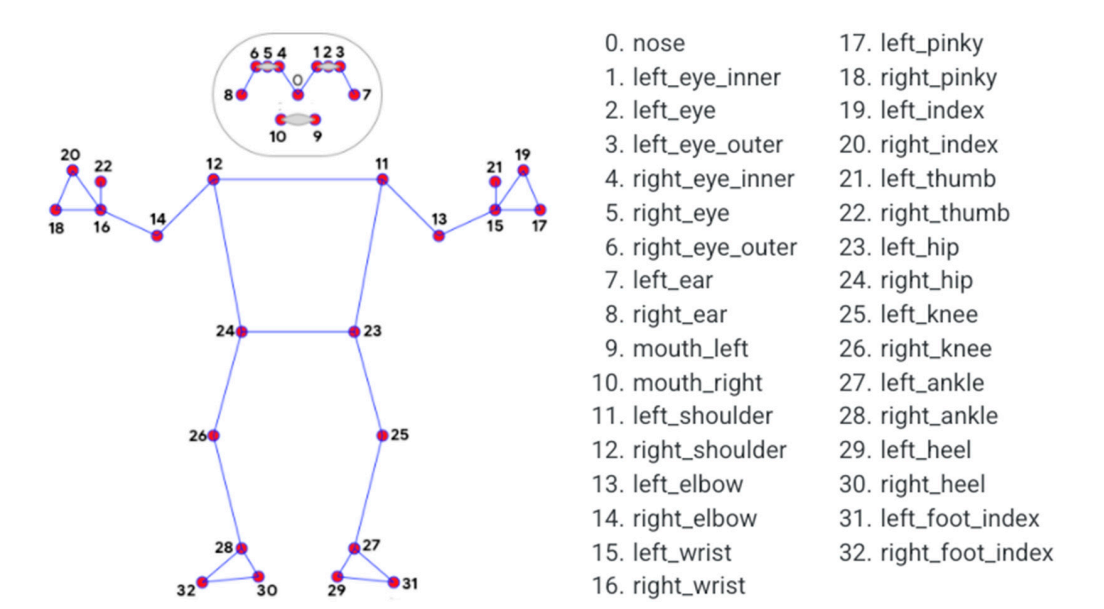
\includegraphics[width=0.9\textwidth]{images/pose landmark.png}  % Menyisipkan gambar dengan lebar setengah lebar teks
    \caption{Defenisi landmark dalam mediapipe pose \cite{bazarevsky2020}.}  % Menambahkan keterangan gambar
    \label{fig:pose landmark}  % Menambahkan label untuk referensi
\end{figure}

Salah satu komponen utama yang digunakan dalam MediaPipe Pose adalah BlazePose, sebuah arsitektur \textit{machine learning} yang ringan dan efisien. \textit{BlazePose} bertanggung jawab untuk mendeteksi 33 landmark tubuh manusia yang mencakup titik-titik penting seperti kepala, bahu, tangan, pinggul, lutut, dan kaki seperti yang terlihat pada Gambar \ref{fig:pose landmark}. Landmark ini digunakan untuk menganalisis dan melacak pose tubuh secara dinamis dalam video, baik dalam mode 2D maupun 3D \cite{bazarevsky2020}.\par

\subsection{\textit{Graph Convolutional Network}} \label{II.GCN}
GCN adalah pendekatan \textit{deep learning} pada data yang terstruktur sebagai graf, yang didasarkan pada varian efisien dari \textit{convolutional neural networks} (CNN) yang beroperasi langsung pada graf.  Model ini memanfaatkan arsitektur konvolusi yang dimotivasi oleh pendekatan lokal orde pertama dari \textit{spectral graph convolutions}. GCN mampu melakukan propagasi informasi fitur dari node-node tetangga dalam graf, sehingga dapat mempelajari representasi tersembunyi yang mengenkode baik struktur lokal graf maupun fitur dari node itu sendiri. Model ini juga dioptimalkan agar skalabilitasnya linear terhadap jumlah edge dalam graf, sehingga cocok untuk graf berskala besar. \cite{Kipf2016}. \par

Secara formal, GCN didefinisikan dengan aturan propagasi per lapisan dengan rumus \ref{eq:propagasi}. \par

\begin{equation}
    \vspace{20pt} 
    \hat{D} = D + I
\label{eq:normalisasi D}
\end{equation}
\myequations{Matriks derajat}
\begin{equation}
    \vspace{20pt} 
    \hat{A} = A + I
\label{eq:normalisasi A}
\end{equation}
\myequations{Matriks ketetanggaan}
\begin{equation}
    \vspace{20pt} 
    H^{(l+1)} = f(H^l,A) = \sigma \left( \hat{D}^{- \frac{1}{2}} \hat{A} \hat{D}^{- \frac{1}{2}} H^{(l)} W^{(l)} \right)
\label{eq:propagasi}
\end{equation}
\myequations{propagasi GCN}

Matriks $D$ dan $A$ masing-masing merupakan matriks derajat dan matriks ketetanggaan, sedangkan $I$ adalah matriks identitas, dan $\hat{D}$ adalah matriks diagonal derajat simpul dari $\hat{A}$. Parameter jaringan $W^{(l)}$ pada lapisan ke-$l$ dipelajari untuk menghasilkan embedding simpul $H^{(l+1)}$ dari embedding pada langkah message-passing sebelumnya $H^{(l)}$, dengan fungsi aktivasi non-linear $f$. Normalisasi $\hat{D}^{-1/2} \hat{A} \hat{D}^{-1/2}$ berfungsi menambahkan sambungan diri pada setiap simpul dan menjaga skala vektor fitur. Selama pelatihan, simpul-simpul yang terhubung dengan bobot sisi yang tinggi akan menjadi semakin mirip ketika melalui beberapa lapisan.


\subsection{Data Graf}

\begin{figure}[H]  % 'h' menunjukkan gambar akan diletakkan di sekitar posisi ini
    \centering  % Gambar dipusatkan
    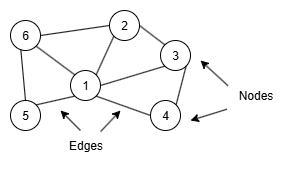
\includegraphics[width=0.6\textwidth]{images/data graph.png}  % Menyisipkan gambar dengan lebar setengah lebar teks
    \caption{Visualisasi data graf.}  % Menambahkan keterangan gambar
    \label{fig:data graph}  % Menambahkan label untuk referensi
\end{figure}

Dalam konteks Graph Convolutional Networks (GCN), graf dapat didefenisikan sebagai struktur yang terdiri dari simpul (nodes) dan tepi (edges) yang menghubungkan simpul-simpul tersebut, seperti yang terlihat pada Gambar \ref{fig:data graph}. Graf ini berfungsi sebagai representasi dari data yang memiliki hubungan atau interaksi antar elemen. GCN memanfaatkan struktur graf ini untuk melakukan pembelajaran yang lebih efisien dan efektif, terutama dalam konteks pembelajaran semi-terawasi, klasifikasi, dan rekomendasi \cite{Kipf2016}. \par

\subsection{Pengukuran Performa Model} \label{II.pengukuran peforma model}
Evaluasi performa model deteksi gerak jatuh pada lansia memerlukan metrik yang dapat menggambarkan akurasi dan kualitas prediksi secara menyeluruh. Beberapa metrik yang umum digunakan dalam konteks ini adalah \textit{Loss}, \textit{Accuracy}, \textit{Precision}, dan \textit{F1 Score}. Masing-masing metrik memiliki peran penting dalam menilai efektivitas model dalam mendeteksi kejadian jatuh pada lansia.

\subsubsection{\textit{\textit{Confussion Matrix}}} \label{confussion matrix}
Confusion matrix atau matriks kebingungan adalah alat evaluasi yang sangat penting dalam bidang \textit{Deep Learning}, terutama dalam analisis klasifikasi. Matriks ini memberikan gambaran yang lengkap tentang performa model klasifikasi dengan menunjukkan jumlah prediksi yang benar dan salah untuk setiap kelas yang dipertimbangkan. Dengan menggunakan \textit{confusion matrix}, peneliti dapat mengevaluasi apakah modelnya cenderung membuat kesalahan dalam klasifikasi tertentu, memberikan wawasan yang jelas mengenai jenis kesalahan yang terjadi dalam prediksi. \par

\begin{figure}[htbp] 
    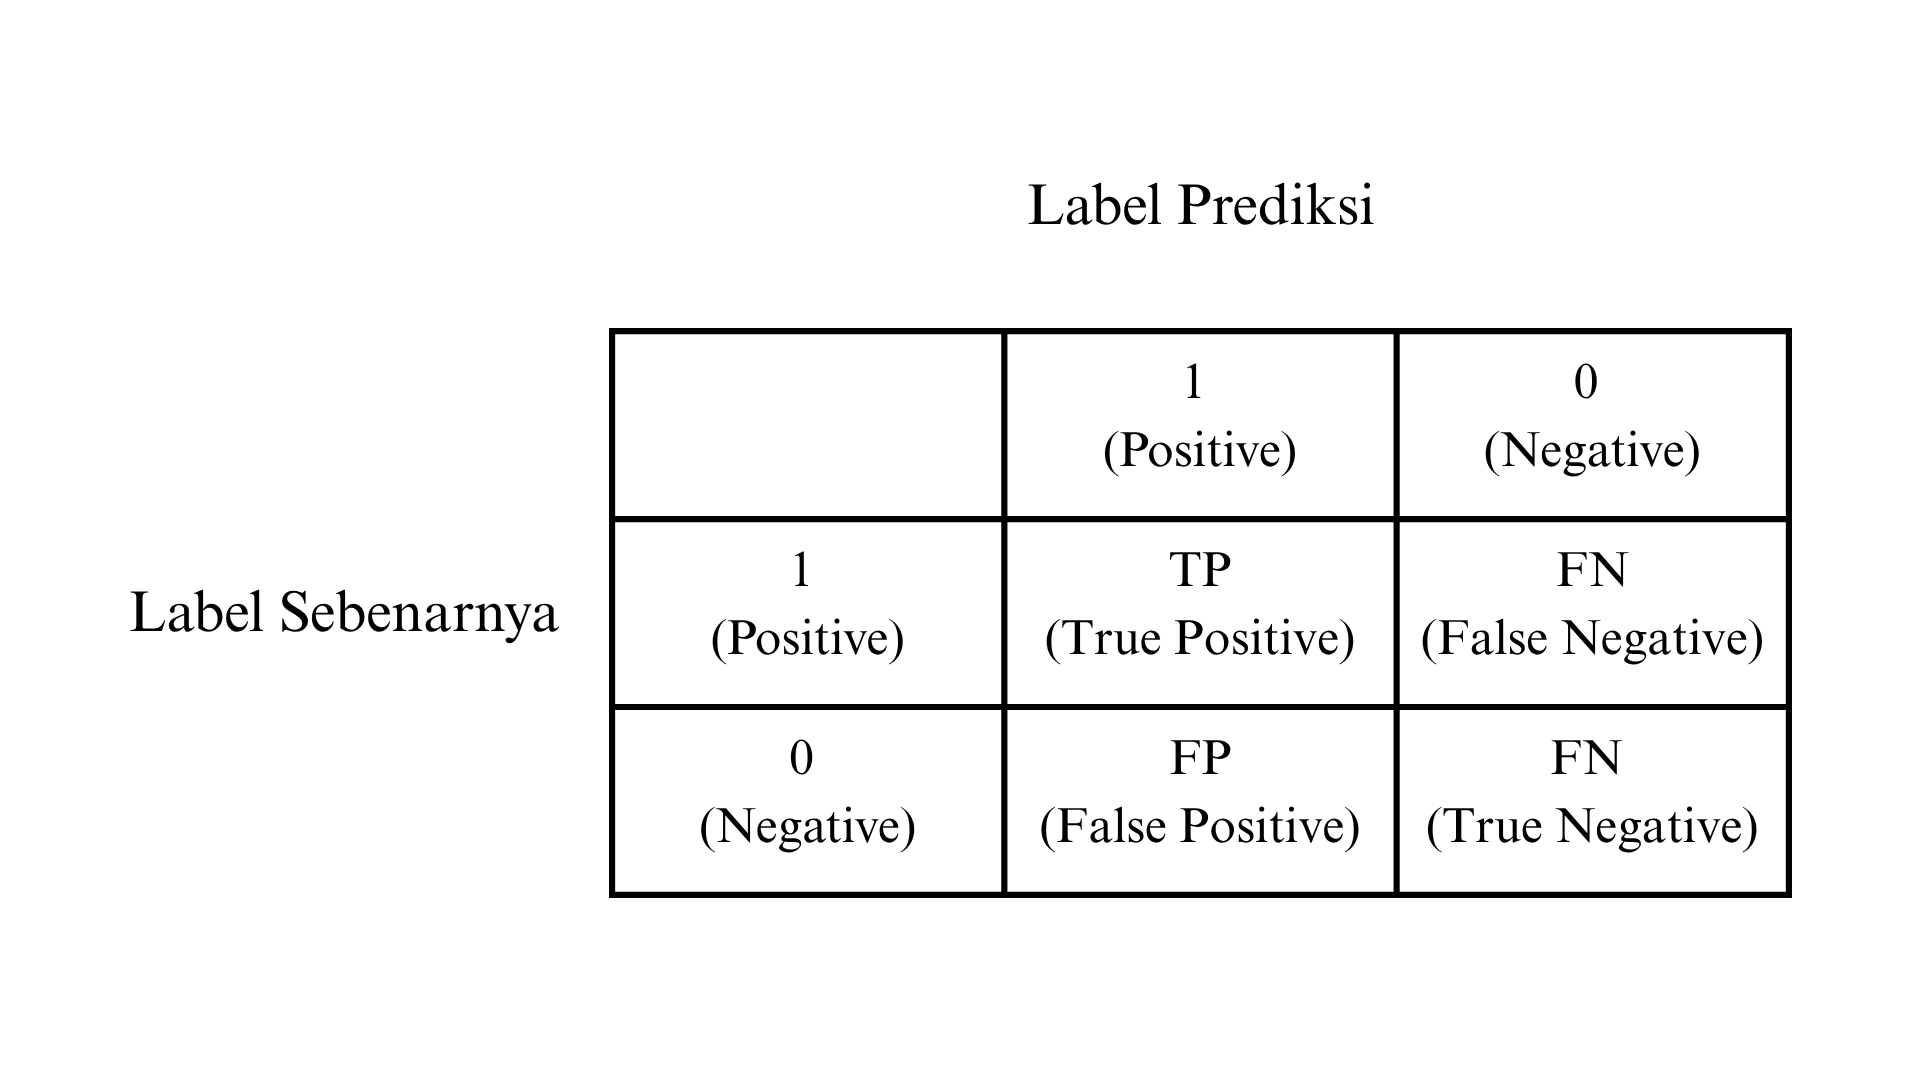
\includegraphics[width=0.9\textwidth, trim={0cm 4.5cm 0cm 4.8cm}, clip,]{images/confusion matrix.png}  
    \caption{Confusion matrix.}
    \label{fig:confusion matrix}
\end{figure}

Tujuan utama dari penggunaan \textit{confusion matrix} adalah untuk memberikan gambaran evaluasi yang lebih mendetail daripada hanya sekedar akurasi keseluruhan. terlihat pada \ref{fig:confusion matrix}, Metrik ini secara sederhana menghitung 4 nilai utama, antara laian.\par 

\begin{enumerate}
    \item \textit{True Positive} (TP): Total prediksi positif yang benar
    \item \textit{True Negative} (TN): total prediksi negatif yang benar 
    \item \textit{False Positive} (FP): total prediksi positif yang salah
    \item \textit{False Negative} (FN): total prediksi negatif yang salah\cite{Albasha2024}.\par
\end{enumerate}
\par

\textit{Confusion matrix} berperan krusial dalam analisa diagnostik, di mana pemahaman yang mendalam tentang bagaimana dan mengapa suatu klasifikasi bisa gagal sangat penting untuk pengembangan model yang lebih baik di masa mendatang. Berdasarkan 4 nilai utama metrik tersebut, terdapat beberapa rumus Perhitungan lanjutan untuk mendeskripsikan peforma model secara lebih mendalam, berbagai rumus itu antara lain 

\begin{enumerate}
    \item \textit{Accuracy} mengukur proporsi prediksi yang benar dari total prediksi yang dilakukan oleh model. Metrik ini dihitung dengan rumus \ref{eq:2.accuracy}. \par
    \begin{equation}
        \text{Accuracy} = \frac{TP + TN}{TP + TN + FP + FN}
        \label{eq:2.accuracy}
    \end{equation}
    \myequations{accuracy}
    
    \item \textit{Precision} mengukur akurasi dari prediksi positif yang dilakukan oleh model. Metrik ini dihitung dengan rumus \ref{eq:3.precision}. \par
    \begin{equation}
        \text{Precision} = \frac{TP}{TP + FP}
        \label{eq:3.precision}
    \end{equation}
    \myequations{\textit{Precision}}
    
    \item \textit{Recall} atau sensitivitas mengukur kemampuan model dalam mendeteksi semua kejadian positif yang sebenarnya. Metrik ini dihitung dengan rumus \ref{eq:4.recall}. \par
    \begin{equation}
        \text{Recall} = \frac{TP}{TP + FN}
        \label{eq:4.recall}
    \end{equation}
    \myequations{\textit{recall}}
    
    \item \textit{F1 Score} adalah rata-rata harmonik dari \textit{precision} dan \textit{recall}, memberikan keseimbangan antara keduanya. Metrik ini dihitung dengan rumus \ref{eq:5.f1}. \par
    \begin{equation}
        F1 = 2 \times \frac{\text{Precision} \times \text{Recall}}{\text{Precision} + \text{Recall}}
        \label{eq:5.f1}
    \end{equation}
    \myequations{\textit{F1-Score}}
\end{enumerate}